%%%% kr2020.tex -- version 1.2 (27-Feb-2020)

\typeout{KR2020 Instructions for Authors}

% These are the instructions for authors for KR-20.

\documentclass{article}
\pdfpagewidth=8.5in
\pdfpageheight=11in

\usepackage{kr}

% Use the postscript times font!
\usepackage{times}
\usepackage{soul}
\usepackage{url}
\usepackage[hidelinks]{hyperref}
\usepackage[utf8]{inputenc}
\usepackage[small]{caption}
\usepackage{graphicx}
\usepackage{amsmath}
\usepackage{amsthm}
\usepackage{booktabs}
\usepackage{algorithm}
\usepackage{algorithmic}
\usepackage{listings}  
\usepackage{enumitem}
\urlstyle{same}
% Copyright 2017 Sergei Tikhomirov, MIT License
% https://github.com/s-tikhomirov/solidity-latex-highlighting/

\usepackage{listings, xcolor}

\definecolor{verylightgray}{rgb}{.97,.97,.97}

\lstdefinelanguage{Solidity}{
	keywords=[1]{anonymous, assembly, assert, balance, break, call, callcode, case, catch, class, constant, continue, constructor, contract, debugger, default, delegatecall, delete, do, else, emit, event, experimental, export, external, false, finally, for, function, gas, if, implements, import, in, indexed, instanceof, interface, internal, is, length, library, log0, log1, log2, log3, log4, memory, modifier, new, payable, pragma, private, protected, public, pure, push, require, return, returns, revert, selfdestruct, send, solidity, storage, struct, suicide, super, switch, then, this, throw, transfer, true, try, typeof, using, value, view, while, with, addmod, ecrecover, keccak256, mulmod, ripemd160, sha256, sha3}, % generic keywords including crypto operations
	keywordstyle=[1]\color{blue}\bfseries,
	keywords=[2]{address, bool, byte, bytes, bytes1, bytes2, bytes3, bytes4, bytes5, bytes6, bytes7, bytes8, bytes9, bytes10, bytes11, bytes12, bytes13, bytes14, bytes15, bytes16, bytes17, bytes18, bytes19, bytes20, bytes21, bytes22, bytes23, bytes24, bytes25, bytes26, bytes27, bytes28, bytes29, bytes30, bytes31, bytes32, enum, int, int8, int16, int24, int32, int40, int48, int56, int64, int72, int80, int88, int96, int104, int112, int120, int128, int136, int144, int152, int160, int168, int176, int184, int192, int200, int208, int216, int224, int232, int240, int248, int256, mapping, string, uint, uint8, uint16, uint24, uint32, uint40, uint48, uint56, uint64, uint72, uint80, uint88, uint96, uint104, uint112, uint120, uint128, uint136, uint144, uint152, uint160, uint168, uint176, uint184, uint192, uint200, uint208, uint216, uint224, uint232, uint240, uint248, uint256, var, void, ether, finney, szabo, wei, days, hours, minutes, seconds, weeks, years},	% types; money and time units
	keywordstyle=[2]\color{teal}\bfseries,
	keywords=[3]{block, blockhash, coinbase, difficulty, gaslimit, number, timestamp, msg, data, gas, sender, sig, value, now, tx, gasprice, origin},	% environment variables
	keywordstyle=[3]\color{violet}\bfseries,
	identifierstyle=\color{black},
	sensitive=false,
	comment=[l]{//},
	morecomment=[s]{/*}{*/},
	commentstyle=\color{gray}\ttfamily,
	stringstyle=\color{red}\ttfamily,
	morestring=[b]',
	morestring=[b]"
}

\lstset{
	language=Solidity,
	backgroundcolor=\color{verylightgray},
	extendedchars=true,
	basicstyle=\footnotesize\ttfamily,
	showstringspaces=false,
	showspaces=false,
	numbers=none,
	numberstyle=\footnotesize,
	numbersep=9pt,
	tabsize=2,
	breaklines=true,
	showtabs=false,
	captionpos=b
}

% Copyright 2020 Florian Idelberger MIT License
% https://github.com/step21/lexon-latex-highlighting/

\usepackage{listings, xcolor}

\definecolor{verylightgray}{rgb}{.97,.97,.97}

\lstdefinelanguage{Lexon}{
    keywords=[1]{lexon, lex, clause, terms, contracts, to, preamble}, % generic keywords 
    keywordstyle=[1]\color{blue}\bfseries,
    keywords=[2]{amount, person, key, time, data, asset, text}, % types; money and time units
    % is|be|certified
    %,|:|;
    keywordstyle=[2]\color{teal}\bfseries,
    keywords=[3]{added, add, subtract, less, greater, equal, le, gt, or, and}, % operators \\+|\\-|\\*|\\*\\*|\\/|\\|\\||&&|\\^|!|<|>|<=|=>|==|!=|="
    keywordstyle=[3]\color{violet}\bfseries,
    keywords=[4]{is, be, certified, certify, may, pays, pay, appoints,},
    keywordstyle=[4]\color{green}\bfseries,
    %,|:|;
    identifierstyle=\color{black},
    sensitive=false,
    comment=[l]{comment, preamble},
    commentstyle=\color{gray}\ttfamily,
    stringstyle=\color{red}\ttfamily,
    morestring=[b]',
    morestring=[b]"
}

\lstset{
    language=Lexon,
    backgroundcolor=\color{verylightgray},
    extendedchars=true,
    basicstyle=\footnotesize\ttfamily,
    showstringspaces=false,
    showspaces=false,
    numbers=none,
    numberstyle=\footnotesize,
    numbersep=9pt,
    tabsize=2,
    breaklines=true,
    showtabs=false,
    captionpos=b
}

% the following package is optional:
%\usepackage{latexsym}

\makeatletter
 \def\@textbottom{\vskip \z@ \@plus 1pt}
 \let\@texttop\relax
\makeatother

% See https://www.overleaf.com/learn/latex/theorems_and_proofs
% for a nice explanation of how to define new theorems, but keep
% in mind that the amsthm package is already included in this
% template and that you must *not* alter the styling.
\newtheorem{example}{Example}
\newtheorem{theorem}{Theorem}
%\texttt{\textbackslash{}newtheorem}

% Following comment is from ijcai97-submit.tex:
% The preparation of these files was supported by Schlumberger Palo Alto
% Research, AT\&T Bell Laboratories, and Morgan Kaufmann Publishers.
% Shirley Jowell, of Morgan Kaufmann Publishers, and Peter F.
% Patel-Schneider, of AT\&T Bell Laboratories collaborated on their
% preparation.

% These instructions can be modified and used in other conferences as long
% as credit to the authors and supporting agencies is retained, this notice
% is not changed, and further modification or reuse is not restricted.
% Neither Shirley Jowell nor Peter F. Patel-Schneider can be listed as
% contacts for providing assistance without their prior permission.

% To use for other conferences, change references to files and the
% conference appropriate and use other authors, contacts, publishers, and
% organizations.
% Also change the deadline and address for returning papers and the length and
% page charge instructions.
% Put where the files are available in the appropriate places.

\title{Merging traditional contracts (or law) and (smart) e-contracts – a novel approach}

% Single author syntax
\author{
    Florian Idelberger
    \affiliations
    European University Institute
    \emails
    florian.idelberger@eui.eu
}

\begin{document}

\maketitle

\begin{abstract}
 For a long time, there have been various parallel developments in the area of AI and Law, Legaltech more recently or computable law, data exchange formats, e-contracts, agreement systems and similar. Some working more on creating normative or logical systems outside of traditional law such as business logic systems, others on bringing probabilistic approaches to reasoning about law or understanding human language, and as an extension, law written in that language. A particular important development are computable contracts, either through DSLs, understanding of natural language or repurposing of other languages such as logic-based languages. In this paper, the most important competitors for writing computable contracts that translate to the environment of a blockchain’s normative environment will be examined in light of their usefulness for creating and merging contracts and e-contracts, functionality and legal looks. Championing the idea that the machine does not actually have to understand anything to be useful, as long as it can comprehensively translate, all the while keeping syntax and semantics intact, making for a more closely integrated contract stack.
\end{abstract}

\section{Introduction}

This work compares several kinds of programming languages that are used and developed for working in conjunction with or instead of traditional legal contracts, compared specifically when deployed upon a blockchain based smart contract system or a similar normative environment.
Different approaches and methods are available, from simple computer code that in effect also has legal implications but isn’t a contract as such and various bridging technologies and (such as SCTs \cite{wongmengComputableContractsAcademia2018}) to the newest advances in writing contracts that have an automatic and accurate electronic representation.
“Legal Tech” in various forms and different comprehensions has been all the rage for a while now, and still is. \cite{braegelmannRechtshandbuchLegalTech2019}  There has been tremendous progress in everything from probabilistic analysis of legal cases to templating systems and contract management systems, as well as the processing of large amounts of cases in specific niches, such as with flight delay claims and similar mass markets. This also brought renewed interest in general AI \& Law/computable law as well as more specifically computable contracts. This work then focuses on computable contracts as understood by Surden \cite{surdenComputableContracts2012}, represented by merging a traditional, natural language legal contract with a smart contract or other e-contract systems. % \cite{othe e-contracting or hybrid systems or delete}
The paper at hand will focus on contract law and specifically a licensing contract for software evaluation. This will be implemented and compared in three different systems. The comparison is made between a direct smart contract language (Solidity) \cite{EthereumSolidity2020}, Prolog \cite{SWIPrologManual} as an alternative declarative, logic-based approach and the Lexon  \cite{diedrichLexonBibleHitchhiker2020} Smart Legal Compiler  using an NLP-like approach and a smart contract templating system.
Each of the approaches will be briefly introduced where after the implementation is introduced, and finally they will be compared and evaluated based on Surden’s criteria and general legal and technological considerations defined more accurately later on.
%There will also be an assessment regarding feasibility and suitability.
After the introduction, there will be a brief ‘primer’ on previous and existing technologies of AI \& law and specifically e-contracting. % \cite{AI & Law - e - contracting}
Thereafter the method and case-selection employed here will be implored in more detail, explaining how implementations were made and tested. Then, the overall case and example license will be presented, where after each implementation is introduced, first by introducing the technology itself and then the implementation that was made. In the end, an analysis is conducted, and a conclusion drawn.
After specially designed programming languages, legal interchange formats and different bridging technologies either with or without smart contracts, new natural-language-like systems present a new frontier for legal programming and e-contracting, merging traditional and electronic contracts. 


\section{Primer on Legal Technologies}
% add citations here?
For quite some time, various technologies for some kind of digitalization of law have been developed under different headings, such as ‘ai \& law’, ‘computable law’ , ‘computable contracts’ , ‘e-contracts’  or ‘smart contracts’ , ‘contract management’, ‘rule systems’, or even very generally ‘legal tech’ which has in recent years become more and more popular with the rise of startups and law firms focusing on legal innovation and digitization. 

\subsection{Legal Markup}
On a basic level of textual representation, there are the systems that structure legal documents, with some tailored towards legislative or judicial documents and others targeting contractual %or other transactional 
documents. This is covered by Legal XML \cite{LegalXML} / Akoma Ntoso \cite{akomantosoAkomaNtosoWhat2015}, LKIF \cite{boerMetaLexXMLLegal} and their variants.

\subsection{Logic-Based Languages}
These are languages and system to reason about legal arguments or outcomes, where logic-based languages are especially prominent.
%, so these will be discussed here.
Specifically, Defeasible logic \cite{nute_defeasible_1993,garciaDefeasibleLogicProgramming2002} was developed as an extension to simple argumentative logic. More widespread and complete languages like Prolog \cite{SWIPrologManual} and ReasonML \cite{ReasonReasonLets}  can be used for similar purposes, such as creating computable law and contracts and reasoning about legal cases.
Part of logic-based languages, expert systems (a precursor of what today is known as 'AI’ or ‘ML’) based on these (or expert systems based on other languages) are ontologies and knowledge bases.  Ontologies  are ‘explicit format specifications of the terms in the domain and the relations among them’ \cite{WhatOntologyWhy}   and a set of instantiated ontological classes constitutes a knowledge base that can be used by logic-based languages or more generally expert systems.

\subsection{E-Contract Systems}
In particular, different evolutions of e-contracting systems can be distinguished. Primarily, there are contract management systems  and e-contracting technologies as such – where the primary aim is merging or integrating legal contractual form, format and structure with some form of technological function and structure. This can be either for just making contracts more machine readable by enhancing them with markup, or all the way up to integrating logic into a document, then automating monitoring and compliance.
%or something in between.
In this paper, the classification specified by Meng Wong \cite{wongmengComputableContractsAcademia2018} % check name
will be employed, where 1st Gen systems are older, proprietary document management and business automation systems,  Second Generation system tend to be newer and more open-source, with many 2.5 Gen Systems having a relation to blockchain based smart contracts and more automation and logic than older systems. Third generation systems are computable law systems such as the CDL/compk  by Stanford (unpublished) \cite{ComputableContracts} and perhaps Lexon. %Contractcode.io, a further example mentioned by Wong, is long since dead and nowhere to be found. 

\subsection{Metadata Systems}
A further, also very important class are meta data formats and systems that process metadata. This is especially very widely used in the area of copyright. Famously SPDX \cite{odenceAdvancingSoftwarePackage2013}  set up a system for open source software packages of all kinds to specify their license, so that licenses can be processed and assessed for compatibility automatically. This has also been adapted or at least been written about to be used in a similar way for other forms of intellectual property, such as in “Computable Law” where Surden writes about SPDX as a way to implement more specific licenses and DRM. \cite{surdenComputableContracts2012}

\subsection{"Legal Tech"}
Finally, practical, modern, commercial examples of ‘Legal Tech’ are companies such as FlightRight  (claims for compensation of delayed flights), WenigerMiete.de  (calculating if you are paying too much rent for your area and helping with claims against that). \cite{ambrogiGoldenAgeLegal2017}

\section{What's legal about code? - The pyramid of norms}
One topic that frequently comes up, and has been discussed numerous times is, if a ‘smart contract’  or another ‘e-contract’  is even a contract in the legal sense. Numerous interpretations narrations abound in literature from ‘of course not, nothing legal about it’ to ‘it will run everything and become sky net’. Fortunately, more nuanced and pragmatic interpretations exist as well.
For the present work, the definitions by Allen \cite{allenWrappedStackedSmart2018}, also used by Cohney/Hoffmann \cite{cohneyTransactionalScriptsContract2020} are used, as they employ a comprehensive understanding of contractual agreement, focusing on agreement and deriving that from a comprehensive ‘contract stack’ which incorporates the textual representation with the layers of natural language and legal language, the program code 
%(‘transactional script’)
and many other utterances that potentially signify intent such as tweets and marketing communication. Whether these are part of the relevant contract stack and are part of defining the intent depends on the specific circumstances and would ultimately have to be decided on a case by case basis. As contracts never exist in limbo or a closed, encapsulated system, this is a solid approach to understanding the nature of smart contracts specifically and e-contracts generally. 
%\begin{figure}
%    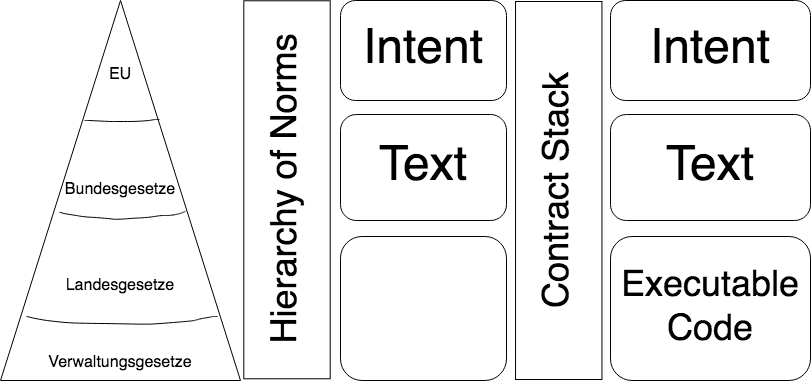
\includegraphics[width=0.455\textwidth]{Contract Stack and Hierarchy of Norms.png}
%    \caption{Hierarchy of Norms \& Example of a Contract Stack.}
%    \label{fig:contract_stack}
%\end{figure}
% Place  all  illustrations  (figures,  drawings,  tables,  and  pho-tographs) throughout the paper at the places where they arefirst discussed, rather than at the end of the paper.They should be floated to the top (preferred) or bottom ofthe page, unless they are an integral part of your narrative3This is how your footnotes should appear.4Note the line separating these footnotes from the text.
% When placed at the bottom or top of a page, illustra-tions may run across both columns, but not when they appearinline.Illustrations  must  be  rendered  electronically  or  scannedand  placed  directly  in  your  document.They  should  becropped outside latex, otherwise portions of the image couldreappear during the post-processing of your paper.   All il-lustrations should be understandable when printed in blackand white, albeit you can use colors to enhance them.  Lineweights should be 1/2-point or thicker.  Avoid screens andsuperimposing type on patterns, as these effects may not re-produce well.Number illustrations sequentially.  Use references of thefollowing  form:  Figure  1,  Table  2,  etc.   Place  illustrationnumbers and captions under illustrations.   Leave a marginof 1/4-inch around the area covered by the illustration andcaption. Use 9-point type for captions, labels, and other textin illustrations.   Captions should always appear below theillustration
The term contract stack is especially fitting, as it can similarly be used to describe traditional contracts that do not have an executable part, as their interpretation in case of doubt also is sought elsewhere. It is also very similar to the ‘legislative stack’ where communications and especially remarks in preparatory documents are used to gage intent. While there is no clear overarching hierarchy in a contract stack, 
%there is still some hierarchy, or at least 
it can be derived in a specific case, such as that text and executable code are probably always higher in rank than intent signified by marketing communication. 
%In Figure 1, a visualization is provided with stack parts provided in order of abstraction or ‘executability’, with marketing communication and other indirect communication at the top, textual, traditional contracts in between and executable parts at the bottom. This is contrasted with the legislative stack.
For the present work, this analogy is important as it frees the later analysis of the specific decision whether a particular instance of textual contract, executable code and other communication or a part of those constitutes a legal contract at a given or all points in time, in a given or all jurisdictions, as the only important conclusion is – it can  – in principle.

\section{Method}

In this section, the method and case selection will be described, meaning how (and why that way) technological solutions were compared and how those that were chosen were selected.
To evaluate the suitability of techniques and compilers this work builds on previous work  where a simple license for evaluation of a product was described in natural legal language, then implemented with Solidity and in defeasible logic. In that case, there was a much more detailed investigation of contract theory, and in the end a focus on the benefits of declarative specification. \cite{governatoriLegalContractsImperative2018} However, it is assumed that because all relevant judicial jurisdictions allow many different forms of signifying contractual intent and agreement, that the model of the ‘contractual stack’ by Allen \cite{allenWrappedStackedSmart2018} holds, and thus while there %will be and 
are certainly differences, 
%for the present examination the intricate differences do not matter most of the time. 
these can be disregarded for this exercise.
%Nonetheless, this comparison of different ways of contractual writing and ‘contractual programming’ is the best way to compare different ways of e-contracting further.
From a legal point of view, depending on jurisdiction there is a definite distinction between license and contract, especially in the United States.
% dist btw license contract
In Germany on the other hand for example, a license is just a different type of contract. For the example presented here, no specific jurisdiction is assumed, although a contractual nature of the license is presumed. \cite{guadamuzComparativeAnalysisCopyright2013}

Compared to the past work, the license example is extended to make for a more realistic testcase. %It is more realistic because it was compared to realistic licenses and adapted accordingly. 
Most importantly, it was extended to include an actual license grant, header with all the participants and a licensing and breach fee. Additionally, to make it more suitable to an e-contract, an arbiter was added so that in case of a dispute, an external party can judge the facts. Finally, the ability to sublicense was added to mirror the licensing example used by Surden. \cite{surdenArtificialIntelligenceLaw2019} These additions add a minimal increase in size, as is relevant for publication, but maximize the usefulness and completeness of the license example.
%For the specific work, 
After a description and explanation of the license at hand and more detailed explanation of its legal nature, the implementations will be presented, such that first the technology itself is described for general understanding and analysed as to its relevance and its specific features that are employed for the task at hand, after which the relevant implementation is presented.
To start, the license example is implemented in a current version of solidity.  \cite{EthereumSolidity2020} This programming language was chosen because it is still the primary programming language for Ethereum  smart contracts (and some others).
%, despite alternatives being discussed and developed. 
Secondly, the license example is implemented in Prolog, \cite{SWIPrologManual} a logic based language popular for knowledge bases, natural language work and pseudo-code. This was chosen as opposed to Defeasible Logic \cite{governatoriLegalContractsImperative2018} or another logic notation as it is much more popular, more easily accessible and reproducible and last but not least with SWISH/SWI-Prolog as a public implementation, the code can easily be tested and run.
%Thirdly, the current status of SCT systems is assessed briefly.

%\begin{figure}
%    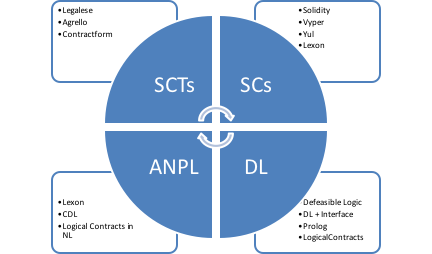
\includegraphics[width=0.5\textwidth]{e-contracting.png}
%    \caption{The main technological stacks of computable law and computable contracts, grouped by kind.}
%    \label{fig:e_contracting}
%\end{figure}
Finally, the same license example is implemented in Lexon \cite{LexonTech}, a next-gen legal compiler merging legal contracts with smart contracts %(or other e-contracts) 
– without losing NLP-like semantics and information of natural language, while gaining substantial automated powers. This compiler was chosen because it is currently at the forefront of merging legal contracts and e-contracts. It combines the clarity of declarative systems with the possibilities of smart-contracts and thus is great to differentiate against Prolog and Solidity.
Finally, in the analysis, the different systems and technologies are contrasted in more detail, based on the criteria by Surden and Cohney/Hoffman. \cite{cohneyTransactionalScriptsContract2020}

\section{Test Case}
A textual test case of a license contract is put forward, that is then used to evaluate against all the technological implementations later on. It is presented in a similar way as the implementations but focuses more on legal aspects.
%as all the other technological implementations.
%, first talking about the technology, then talking about the precise implementation and the specific test case as such, though necessarily focuses more on the legal aspects.
\subsection{Textual "Technology"}
The most common and ordinary use of contracts is still by ordinary language, written or spoken words in a given natural language that can be enriched with legal jargon and terms specific to a particular field or industry. The ‘medium’ is often a piece of paper, but one particular feature of the law is that its medium or articulation are of lesser importance unless otherwise prescribed. %Thus, this is the starting point and reference point.
\subsection{Test Case}
%\lstinputlisting[caption={License for the evaluation of a software product}, language=text]{license.txt}
\begin{example}\label{ex:license_example}
This license is an example evaluation license.

\begin{enumerate}[label={Article \arabic*.},leftmargin=*]
%\begin{lstlisting}[language=]

\item[] LICENSEE - The University
\item[] SUBLICENSEE - A student as set force in the appendix. (array of persons)
% enrolled in a major % relevant to the field % that benefits from journals 
\item[] ARBITER - An arbiter or oracle that decides in case of disputes. Can be a natural or legal person or a machine. Art. 2, 3 and 4 especially are evaluated by the arbiter in case of disputes.
\item[] ASSET X - An asset to be licensed.
\item The Licensor grants the Licensee a license to use and evaluate asset X and grant sublicenses among group Y, for use and evaluation. This grant is in exchange for a licensing fee.
\item (optional) The (Sub)Licensee is commissioned to publish comments about the use of the product. This allows publication of comments but also requires them.
\item The (Sub)Licensee must not publish comments of the use and evaluation  of the Product without the approval of the Licensor; the approval must be obtained before the publication. If the Licensee publishes results of the evaluation of the Product without approval from the Licensor, the Licensee has 24 h to remove the material.
\item Article 4.  This license terminates automatically if the (Sub)Licensee breaches this Agreement. Breach obliges the licensee to pay a fee to Licensor for Breach of the Licensing Terms.
\end{enumerate}
%\end{lstlisting}
\end{example}
The test case is a license contract to license a copy of a software or other specified work for use and evaluation, in exchange for a licensing fee. Furthermore, sublicensees can be specified. These grants and license are defined in article 1. The sublicense part was inspired by Surden’s  description of a licensing system where universities can automatically manage the licenses of their libraries and conclude more tailored licensing agreements. %It also adds an interesting dimension to the test case, where potentially huge swaths of sublicensees have to be defined.
In article 2, it is defined that optionally, the licensee or sublicensee is commissioned to publish comments about the use of the product. This %then
approves publication, but also requires it. %This, in conjunction with changed language, clarifies the distinction between publishing and commenting in the earlier work that this paper was inspired by. 
In article 3, publishing of comments about the use and evaluation of the asset without approval by the licensor beforehand is prohibited.
%may not be published without the approval of the licensor, obtained before publication.
%it is defined what not to do, specifically, comments about the use and evaluation of the asset may not be published without the approval of the licensor, obtained before publication. 
In case of unauthorized publication, %without approval, 
the licensee has 24 hours to remove the published material. This improves %and hardens 
the test case, as it %likely 
requires use of external agents or data sources depending on the system, as otherwise there is no basis on which to automate or act. Additionally, the passing of time is tested with the time limit.
Finally, in article 4, it is laid out that the license agreement terminates automatically upon breach of the licensing agreement, and that the licensee has to pay a fee in case of breach.
The resulting license agreement is simplified for publication, but includes the most important features of license contracts.
%also held brief for publication, is simple but includes and tests the most important factors of most (license) contracts.

Compared to the previous work, this example adds important features that make it an actual license. %Most importantly, 
The asset that is licensed is defined and the relation between commenting and publication and how this relates to the possibility of the licensee being commissioned by the licensor is clarified.
%or at least can be defined. Furthermore, it is important to clarify the relation between commenting and publication, and how this relates to the possibility of the licensee being commissioned by the licensor.
In reality however, this would still be defined differently, with likely a statement of intent, the spirit of the license in the beginning and much more detailed definitions. Last, it was not clearly defined when the license was breached or would be terminated, so that was improved. %This has also been improved but could also still be better.
In order not to make it too hard on the example implementations, some care is taken that the licensing contract does not constitute or seem like an impossibility. To this end, it was evaluated on the basis of Surden’s criteria for computable contracts. \cite{surdenArtificialIntelligenceLaw2019}
According to Surden, most of all a computable contract needs some kind of data source, to assess performance, compliance or breach, which then lead to lower transactions costs and increased reliability. Additionally, the computer or the contract on a computer needs to be told what to do, which Surden calls an ‘automated prima facie assessment.’  In the example, the main points in this regard are the granting of the license itself, the determination of when or how an evaluation and or comments were published, if they were removed in time and finally whether or a given set of facts with regard to these licensing obligations constitutes a breach of contract or not. While parts of this can be automated, in such a general textual form, not all of it can. Thus, to give the computable contracts a fighting chance, an arbiter is introduced to help make determinations. The arbiter is a natural or legal person or possibly also a third-party software agent that can make determinations about facts in case of disagreements. %, to introduce offline data into the online world.
The resulting test case license is still % very
imperfect, but an actually used license in natural, legal language probably could fill a whole paper on its own. In Surden’s case with SPDX \cite{odenceAdvancingSoftwarePackage2013}, this license is relatively well suited for computable contracting, as much more fine grained licensing is possible, thanks to being able to define (sub)licensees based on criteria of the student population, clear delineation of the asset being licensed and the parties involved, with a limited number of happy states and failure states.
It is furthermore assumed that the actual object of the license is described either in the license, by a graphical interface or extracted from business logic systems. Thus, (sub)licensees are easily accessible, and license status and publishing obligation or permit are available.

In the spirit of Surden’s assessment, this presents a good starting point for our experiment of examining different license implementations, as he claims computable contracting is limited by possibilities of automated assessments, but which he claims goes ‘far enough’ more often than not.

\subsection{The criteria of examination}
In earlier work the focus of comparison was on detailed legal theoretical comparison, describing the contractual theory of contracts as ‘legally binding agreements’  with the core tenants of the agreement of the parties, consideration in exchange for something, the competence and the capacity of the parties involved and the legal object and purpose of the agreement. \cite{governatoriLegalContractsImperative2018} %Furthermore legal interpretation and lastly the ‘Lifecycle’ of a contract were discussed. % life cycle stuff was deleted here
%These are all important issues, but f
For the present analysis, the focus is on whether the test case and its implementation capture the meaning and spirit of the contract (as well as syntax and semantics), are functional and most of all still ‘look like a contract’ and can be read and understood by legal professionals and others alike. 
%Some aspects of the lifecycle are still relevant, however are also mainly an implementation issue. 
Now, with the stage set and the criteria explained, let’s meet the candidates of this event.

\section{The implementations}
The e-contracting implementations are presented and assessed. While they are assessed on the basis of a smart contract system, they could %often
also be implemented to work with another e-contracting systems or more general normative environments. 

\subsection{Solidity}
As an example of an imperative language that is used to program ‘e-contracts’ Solidity is used, which was the first higher level language for such scripts in the blockchain space, and is still dominant at the time of writing. \cite{SoliditySummit20202020}
\subsubsection{Technology}
The solidity language was established by the Ethereum project. \cite{gavinwoodEthereumSecureDecentralised} It is an imperative %and compiled 
language that compiles down to bytecode that is run in the Ethereum Virtual Machine (EVM), borrowing somewhat from JavaScript in syntax, but otherwise being statically typed and otherwise constrained due to the execution environment on the blockchain. This is due to the fact that as the code is necessarily computed by miners when proposing new blocks for the blockchain, it has to be ensured that the output is always the same given the same input and infinite loops or DDOS attacks are to be avoided.% or at least should be made harder.
This necessitates strict typing, (relatively) fixed arrays  and very strict loops that do not run an indeterminate amount of time. For this, each execution step is priced in terms of ‘gas’ in the EVM, which puts an extra cost on complex programs, but especially on storage. The language is relatively readable, but only in so far as traditional programming languages go. The gas system is imperfect and flawed, but the best solution available so far, using economic forces to secure its network.
%also going in spirit with the ‘economic system’ of a market based technological system established first with Bitcoin and improved with Ethereum and the gas system. %This might change in the near future with the testing and then launch of Ethereum 2.0 which will switch from a mining-based system to another system, that is also built on incentives and disincentives, but more scalable and with different assumptions and incentives. (see below)
%Functionality => lifecycle

\subsubsection{Implementation}
This is an implementation of the license agreement in solidity, with a current version of solidity as of this writing. A lot of space is captured by the simple definition of basic variables and their types. These are necessary for functionality at one hand, and for EVM execution on the other hand, as a system with execution constraints such as the Ethereum Smart Contract system needs this information to price execution and storage. There is also a certain amount of inherent duplication – f.e. it can be seen that variables established for the contract have to passed again to the constructor %(which establishes how and what is necessary to deploy and instantiate a contract) 
whereas these variables are necessary for the solidity language, they do not serve any purpose in conveying the legal or natural meaning of a contract with regard to the agreement and the ‘spirit’. 
However, it can at least be said that a properly written smart contract
%or ‘transactional script’ 
in an imperative language such as Solidity does achieve a lot of functionality. For the functionality, it can f.e. be held that important events such as contract creation, termination, mediation (via arbiter), performance and modification as well as monitoring can be automated, or at least made partially functional, %depending on what is wanted, 
using such a language. This might seem obvious,
%is of course maybe obvious
as that is the purpose of the language, but it will 
%later on 
become visible that in the comparison performed that is a very relevant distinction.
Finally, it is fair to say that no normal legal professional or layperson would even begin to understand the meaning of such a contract or script. Even for some programmers, or smart contract developers even, it can be very hard to fully understand the meaning and all nuances of smart contracts, as has repeatedly held in previous literature. 
\lstinputlisting[language=Solidity, caption={This is the Solidity Implementation of the License.}]{license_new.sol}
Further, it is on one hand more prone to errors, and on the other hand much more verbose
%and in some cases much easier to read, 
as the format is much more visible. In an actual blockchain use case, especially on a 
%normative 
system with such economic incentives,
%\cite{gas} 
it would probably also make sense to implement a lot of actual evaluation off-chain, because as long as license data is on-chain, it can be safely checked off-chain by ‘everybody’. Still, this would necessitate some other connection between legal contract, structure and semantics and the functional transactional scripts. Thus, ideally, independent of characterization of ‘smart contracts’, there would be a stronger link between the legal part of a smart contract and the functional parts of it. The surrounding environment anyway has to be adapted to contract management systems or end user needs, but a human readable contract that captures the contractual essence is in both cases an asset.

\subsection{Logic-based languages (Prolog)}
Whereas the previous work \cite{governatoriLegalContractsImperative2018} focused more on legal lifecycle and logic-based languages as such, with a strong focus on Defeasible Logic because its built-in ‘defeasibility’ lends itself well to contracts that have no ‘undefined’ states, the present work uses Prolog due to accessibility and availability, ease of replication and suitability due to great previous work testing the limits of Prolog for legal reasoning and logic.
%Prolog is here used as an example for various kinds of attempts at using primarily logic-based languages for contract like systems or generally reasoning about law and contracts. Reasoning is here understood as making deductions based on a set of inputs.

\subsubsection{Technology}
%A logic-based language (DL) was in the past already evaluated for use as a smart contract language due to its unique defeasible properties, that allow for conflict resolution between rules.  However that comparison focused very much on the languages as such, to some degree comparing apples to oranges if you will, not taking into account their different environment that makes a straight comparison unhelpful.
Prolog is here used as an example for various kinds of attempts at using primarily logic-based languages for contract like systems or generally reasoning about law and contracts. Reasoning is here understood as making deductions based on a set of inputs. Furthermore, the syntax and structure of Prolog is more easily acquired and tested. %For comparison, one line of Defeasible Logic is compared with one line of Prolog.

%\begin{example}\label{ex:dl_vs_prolo}
%Direct comparison of DL vs Prolog
%\begin{enumerate}[label={},leftmargin=*]
%\item[] \verb|Art1.0: => [Forb_licensee] use|
%\item[] |vs|
%\item[] \verb|use(Licensee, forbid)|
%\end{enumerate}
%\end{example}
%\begin{example}[How to write an example]
%Examples should be written using the example environment defined in this template.
%\end{example}
%\begin{algorithmic}[H]
%\begin{lstlisting}
%Art1.0: => [Forb_licensee] use 
%\end{lstlisting}
%vs
%\begin{lstlisting}
%use(Licensee, forbid)
%\end{lstlisting}
%\begin{lstlisting}
%"Art1.1 > Art1.0" vs ??
%\end{lstlisting}
%\end{algorithmic}
%“Art1.0: => [Forb_licensee] use” vs use(Licensee, forbid)
%“Art1.1 > Art1.0” vs ??

%So instead, for the modified license, a Prolog implementation was made. Prolog is a declarative logic-based language, primarily designed for ‘logic programming’  and natural language processing, and heavily influenced by research about resolution mechanisms and methods for extracting answers.  When used to algorithmic or imperative programming, Prolog takes some time to get used to think in the different paradigm. Still, despite its different mode of working, it still has quite a few input / output characteristics and data structures of general programming languages.
While Prolog is not as tailored to be defeasible and can in principle have unclear states, it otherwise supports everything that DL supports and even much more. \cite{morelliralphPROLOGFactsRules}
%Most importantly however, it is much more accessible, meaning that everyone can test the provided listing in seconds in a web browser or on a desktop computer. While there are many implementations available, because of availability and widespread use, SWI-Prolog  was used.

The main parts of Prolog used in this research are facts ‘exists(paper).’, which means paper exists, rules denoted by ‘:-’ which evaluate the left statement to true if the conditions on the right hand side below match, and variable, denoted by every term starting with a capital letter. As the Prolog interpreter, similar to a DL implementation %or many similar systems  
does by default not know anything, everything has to be provided, which also means that some basics are just facts that are assumed to be true or set by the creator as true, as otherwise there would be no starting point. This is opposed to a blockchain based system or many procedural languages, where for example an identity structure or similar might already be implemented.
% thus prolog making things more explicit, as ofc also base of other system has implicatons/biasis etc
%It should be noted that it would also be possible to write a more complete Prolog program that for example asks for input or complains if some necessary facts to answer a question are missing, however that would be an implementation concern and out of scope for the present work.
Overall, it can be concluded that Prolog is very useful for sketching logic and processing workflows and can easily be accessed. Care should be taken to make sure the supplied answers make sense and the names or words used for naming variables and facts actually make sense, as compared to imperative programming, the supplied facts and rules are not merely variables but actually make up the knowledge base of the project, such that badly named, too short or too long items can render the whole project hard to read or even useless.
For actual implementation however it would probably be seldom used, as too much would have to be written around it. That could be different with more tailored variants such as DR-Prolog \cite{antoniouDRPrologSystemDefeasible2007}, LogicalContracts \cite{LogicalContractsAlpha} or if translation to an imperative language becomes possible, that can directly be deployed in a normative system where its facts take on deeper meaning by being connected to identities, values and assets.
Thus, at the very least for testing, Prolog and similar languages are very relevant, though it would help to have a system on how to set facts, verbs and rules, as otherwise inputting knowledge can seem arbitrary. 
% Implementation smart contracts? 

\subsubsection{Implementation}
The Prolog implementation of the textual license example mentioned above can be found below.
First, similar to the preamble of the textual License, some basic facts are laid down, such as the natural or legal persons that are a part of the license, if the Licensor commissioned the Licensee and if the comments of the evaluation were published or not and how long ago that was. %These could be omitted, but then would have to be supplied at runtime, so with the goal of publishing a version that resolves, they were included in this version.

In article 1, the licensee is granted a license by the licensor, and it is checked if both parties exist, whether a fee was paid and if there actually was an offer of a license. If either is not true, there is no license. Furthermore, if there is a license, sublicenses are allowed, and it is defined that the licensee may publish comments in case there is a license and the licensor approved the comments.
%permitted the comments?
Afterwards, in article 2 it is defined that the licensee counts as commissioned in case the licensor commissioned them, and that if they are counting as commissioned, they also must publish the comments.
Thirdly, in article 3,  the prohibitions are laid down, whereto the licensee may not publish comments if they were not approved and that they must remove them if they do it anyway and with an extra check of the time, so that this obligation to remove disappears in case it is complied with.
Finally, in article 4, it is established that the license terminates if there is a breach by the licensee, and that the licensee has to pay a fee in case of a breach.

The biggest issue with pure logic-based examples is mainly their lack of grey areas and how they learn about facts. %This is also an issue for smart contracts, if they need to know facts outside of their normative system.
How these facts get there – also a big issue with smart contracts in general and solidity in particular  – is not solved, so the great properties of a logic-based implementation are always limited by its surroundings. 
Thus, this only solves the actual logic. The actual input/output still would have to come from somewhere else, an
%so this means there is an 
additional layer of implementation for any logic-based use, where errors can be introduced and part of the advantage of the logic-based approach gets lost in the process. %unless these layers can be incorporated into that approach, such as using a declarative language. 
Declarative languages used for functionality could help, however it is uncertain if that will really help, as truly self-contained languages are probably too limited, any introduction of uncertainties will make the logic-based approach also more error prone
%, even if only at the fringes of implementation.
\lstinputlisting[caption={This is the prolog logic version.}]{license.pl}
For logic-based approaches, they can capture most of the meaning and spirit of the contract, however it will only be accessible by experts. Even if it is more precise than imperative programming, languages such as DL and Prolog are still too arcane to fully capture a contract and make it accessible. Partially, this is because the intricacies of syntax and semantics of natural language are not captured in the kind of logic-based ‘contract’ compared here. The resulting work is functional, in so far as questions can be asked of it, it can be resolved for facts and answers like an equation, and it can be automated and supplied with data in much of the way that Surden envisions. Still, it does not really ‘look’ like a contract and as said in the beginning would need some connection to a different textual version of the contract to be accessible %for laypersons and legal experts, 
thereby negating most benefits.
%For other, possibly different solutions, Model Checking Contracts (Imandra)  and LogicalContracts  should be looked at.

%\subsection{SCT-Systems}
In what Wong calls the 2nd generation of Smart Conctract Templating Systems and their blockchain brethren in the 2.5 generation, no winner has emerged yet, even of those that are still alive. Due to space constraints, this discussion is omitted here.
%In the wake of Blockchain technology in general and e-contract / smart contract excitement more specifically, especially during the ICO  hype of 2017, a set of technologies emerged that all tried to bridge traditional contract texts and either blockchain smart contracts or other kinds of ‘digitalization’ of written contracts.
%These are mostly templating systems and similar technologies, as described in much more detail by Wong.  In the scope of this paper, the classification by Wong will be used. He distinguishes between 1st Generation Document Assembly Systems, Smart Contracts per se, (Smart) Contract Templates and Smart Contract (Templates). These he then categorizes into 2nd Generation templating systems, 2.5 Generation “Bridges” and 3rd gen systems. If we see them through the lens of the term of a ‘contract stack’ established by Allen, the 1st generation systems were merely electronic template systems to assemble documents (and proprietary according to Wong etc) and thus lead to an assembled final textual version with no automated or functional component. The 2nd generation system such as CommonAccord and CommonForm draw their inspiration from open-source and are widely geared towards ease of sharing, interoperability (such as generation of diff file formats) but are otherwise also quite fixed on the textual, legal language based layer, except making it more accessible and processable through variables and public specifications as opposed to closed systems.  (in fact Wong wrongly categorizes CommonForm and CommonAccord as first 2nd Gen and then 2.5 Gen, but there is currently no evidence of that. While CommonAccord mentions blockchain on its page, the templating system seems to be wholly independent of that) 
%In Wongs classification, 2.5 Gen systems then incorporate some kind of bridging technology, between text and executable or other technological parts, such as executable blockchain code. One simple version of that might have been Legal Markdown of Eris Industries (since abandoned), which was one of the first in the blockchain space, where text could be linked with a software version via a hash of the document and a hash of the smart contract. However, it seems that this distinction is too indistinctive, as 2nd gen systems already had differing features and to establish half a new version just because of the ICO hype in 2017 or many felt the need to add seems not a good basis for a classification anymore. Where this distinction might be relevant, is systems/projects that were established just because or at least in the blockchain and ICO/smart contract hype. As such, below an update table will be presented that presents an up to date take and view on the state of the projects (with some additional ones) that Wong reviews.


%Regarding 3rd gen systems, such as Compk  from Stanford (dead in the water so far) and contracode.io (even more dead, with not even a website anymore) Wong identifies a DSL as the main distinguishing feature of a 3rd gen system. Due to lack of an actual 3rd gen system, this is hard to judge. The closest right now might be Lexon described below and LogicalContracts (above, based on Prolog), though it is unclear into which direction LogicalContracts are developing. As part of a contractual stack, templating systems or other methods such as user interfaces generated from them are definitely necessary and will be a part of any contractual stack that aims to be comprehensive and incorporates traditional legal work.


\subsection{Lexon}
Finally, Lexon is described as a primary example of a new kind of ‘script’ specific to e-contracts, developed specifically for merging e-contracts and legal contracts, while being easy to write and read for humans without requiring huge computing resources.
%such as natural language processing (NLP) systems trying to understand language properly. 
\subsubsection{Technology}
Primarily, Lexon \cite{diedrichLexonBibleHitchhiker2020} resembles the structure of legal contracts, and uses similar language. It is already functional but at the time of writing also still under heavy development. The defining unique characteristic is that it uses direct translation of natural language and legal prose to executable code via an Abstract Syntax Tree, without a secondary intermediary layer. This keeps the structure and syntax and higher order meaning of the original document much better. While Lexon documents require a certain structure, it is not foreign to people nor lawyers and very natural language like.
%, claiming to use the AST to infer the intent of legal contracts. 
So far, it comes closest to a
%is the closest example that I have seen of a proper 
3rd generation SCT system, according to Wong’s definition of the main characteristic being a DSL \cite{wongmengComputableContractsAcademia2018}, although with the aim to go even further.
%and an actual DSL that does not look like a DSL. 

Each document starts with a title, mentions the Lexon version it is built for, and can offer some explanation or other guidance in a preamble, similar to a normal legal contract. In a further section, terms are defined, such as the parties to the contract, amounts and fees and what their role is.
Then, the main contract starts via ‘CONTRACT(S)’. The contract is then divided into ‘clauses’ that roughly match onto functions in a solidity coded contract.
	%\texttt{algorithm}
%\begin{algorithmic}[H]
%\begin{example}\label{ex:lexon_clause}
%Direct comparison of DL vs Prolog
%\begin{enumerate}[label={Article \arabic*.},leftmargin=*]
%\begin{lstlisting}
%CLAUSE: Pay.
%    The Licensee pays the Licensing Fee to the Licensor,
%    and the Breach Fee into escrow.
%    The License is therefore Paid.
   
%\end{lstlisting}
%\end{algorithmic}
%CLAUSE: Pay.
%The Licensee pays the Licensing Fee to the Licensor,
%and the Breach Fee into escrow.
%The License is therefore Paid.
%Fig x: Example of a Lexon Clause

This example demonstrates, that first there is the CLAUSE keyword and that Lexon still partly relies on keywords, similar to other, imperative programming languages. However, it was developed in such a way that its keywords are as close as possible to legal language used in ordinary contracts, and its actual content is legible for programmers, legal professionals and everybody else alike.
So far, all the ‘actionable’ words are mapped to terms and phrases in the solidity smart contract language, however in principle they could also map to other normative systems, such as business rule systems.% and similar technologies. 

\subsubsection{Implementation}
Below is an implementation of the license example in Lexon. At the beginning, the header with the name of the contract, the software version and the preamble are shown. Preamble is a non-actionable part of the script but might be very relevant in case of a dispute as earlier literature argued that in most cases there is always a ‘contract stack’ consisting of multiple expressions of the contract, such as the ‘smart contract’ as a functional layer and others that could help with interpretation, particularly with finding out the intent of the agreement and the parties involved. 
%Obviously, strategies and approaches of judges will differ from jurisdiction to jurisdiction, but due to their self-image and status, it can be presumed that judges will not simply say ‘the code is law’ and disregard intent or agreement signified outside of code in the pyramid of e-contracting norms. 
% put this somewhere else, not fitting here?
In the next section, the terms are fixed, defining who licensor and arbiter are, the fees are established and set and an arbiter is appointed. Then, the actual contract is defined, in this case ‘per licensee’ so that it is clear that there is one contract per licensee. This is then also deployed like that later, in that executable code is instantiated with actual amounts, assets and identities per licensee, and certain properties like “Permission to Comment” are established, and most importantly, a description or link to an identifying token for the licensed assets are established. This could be just a boolean, a license key or a hash of the licensed work for example. If and how this would be checked is another matter, in case of software it could be checked by the software itself, in cases of artworks it could be checked via a DAPP or centralized website for such work. For all content of the license articles that have an actually “actionable” function, meaning it can at least to some degree be recorded, automated or delegated to the arbiter, there is a ‘CLAUSE’ that signifies that. When compiled, these would be mapped to solidity ‘functions’, and are also mentally much closer to a kind of ‘declarative function’ then clauses, as they are understood by legal professionals. This is also one of the main negative points, that while the resulting code is much closer to ordinary contractual language, still certain keywords and a certain structure should be used. However, it should also be noted that these depend a lot on the underlying normative system that they compile to, meaning as the underlying system uses ‘functions’ (in Solidity), Lexon needs to map to them. In a different normative system, such as a business rule system, this could be organized differently.

% maybe use minted package instead
\lstinputlisting[language=Lexon, caption={This is the Lexon version.}]{license_eval.lex}

As can be seen, the license as implemented in Lexon is relatively close to the meaning and spirit of the contract, though it still needs a certain structure. The syntax and semantics are close enough to natural language to be readable and require little or no training to grasp meaning and spirit of the contract. Furthermore, the result is as functional as any ‘smart contract’ of the underlying system.
%with potentially the drawback that if a contract coded directly in solidity or even in a lower level language can take more shortcuts (assuming it is still safe) it will save on fees and processing time. 
Most importantly however, the Lexon contract still mostly looks and feels like a contract (and could be made to look more natural as well, i.e. fill words and similar do not bother the compiler) so that it can be read and understood by most, but especially also by legal professionals without programming or other in depth knowledge.
Thus, the Lexon stack is a at least for now quite promising and the most advanced digital contract stack available, being a proper 3rd gen SCT system %and with all-encompassing contract stack 
although it remains to be seen if it will continue to prosper or stagnate and remain an interesting experiment.

\section{Findings}
The investigation started with an example of a software licensing contract, which at one hand includes things helpful for electronic contracts such as a provision for an arbiter, but on the other hand also features time and vague uncertain provisions that require such a change and highlight the difficulties in understanding, interpreting and enforcing contracts, not only but especially when in a restricted environment such as that of a smart contract language.
%One important change to previous work was, that there is an actual license grant and a license fee in the first place, and to make it more relevant to Surden’s example with SPDX, an option to add sublicensees such as students was added. Lastly, the clarification of breach/termination/cancellation and the fee paid makes it also much more realistic while still keeping it short.
If we then compare this to solidity, as representing an imperative, somewhat high-level language, stark differences emerge, as the contract as such is not representable in such a language. Still, even a piece of software, including its documentation, git commit logs and informal communication %(or other ‘informal’ agreements)
can be seen as a contract, as supported %by the investigation 
by Allen. \cite{allenWrappedStackedSmart2018}  The solidity example explicitly describes the actions that the smart contract should support, with a lot of technical jargon and even experienced programmers still frequently get it wrong. This does not mean that Solidity doesn’t have its uses, however it has to be taken into account. It is also observable, that there is a lot of repetition in the smart contract, such that not only does a variable have to be initialized, but then it has to be passed to each function and the constructor as well, causing a lot of extra text especially when trying to use descriptive variables and function names. An additional difficulty could arise due to scoping problems – meaning that like in other languages, variables have a local, global or possibly other scopes, such that variables can have different meaning and values depending on where they are. This could maybe be related to context in natural language, but there, people and legal professionals are used to it and there is context, in the context of %an unknown world like 
a programming language it is just foreign and the context is more akin to two brackets instead of three.
If defined in terms of the contract stack and our criteria established above, the solidity implementation gets full points in the functionality department, as everything that is possible in principle within the constraints of the Ethereum EVM is possible. It also at the very least has the possibility of the ‘meaning and spirit’ of a contract.
%though sometimes the actual agreement is only established on user interaction with the contract. (such as a licensing contract on the blockchain, that I send a certain amount of currency in addition to the id of a song that I would like to license). 
In regard to syntax and semantics, a Solidity based contract does not really capture the nature of the original license contract, and neither does it ‘look like a contract’ to legal professionals or laypersons. Lastly, the contract is also not read nor understood by them.
In the next section, %logic-based languages were looked at. Specifically, 
Prolog was looked at, a widely available, accessible and extensible, logic-based language. 
%Prolog was chosen as opposed to more specific offshoots, as it is much more accessible and reproduceable, and the high cost of accessing a niche language such as DL or DR-Prolog or similar outweighed their benefits. 
First, also the Prolog example captures the meaning and spirit of the contract. The syntax and semantics are much more reasonable and readable, and it looks a lot more like natural text, still not like a contract though. However, a big problem is that in general, logic-based languages, including Prolog, offer a lot of flexibility, but without the flexibility and dictionary of natural language. As a result, much depends on the choice of terms and verbs, %(or if verbs are even used at all) 
and on the understanding of the definition of facts, variables and functions/rules in Prolog. More specifically, facts and rules can be very detailed and specific and easy to read depending on how they are chosen, but can also be very useless, if cryptic or confusing terms are chosen.
%And the part about facts and rules means that the meaning of x(y) (y is x), := (rule) and capitalized terms (variables) has to be understood.
This makes it maybe even more confusing than an imperative programming language, as the differences are more subtle and a system for defining facts and rules would be necessary to have a certain predefined standard.
%\begin{example}\label{ex:logic_standard}
%Example of different logic-based notation of predicates.
%\begin{enumerate}[leftmargin=*]
%\begin{lstlisting}
%\item[] \verb|is_commissioned(license)|
%\item[] vs
%\item[] \verb|commissioned(license)|
%\end{lstlisting}
%\end{enumerate}
%\end{example}
Furthermore, a logic-based contract is ‘solvable’ in the sense that the interpreter can solve it based on input and determine possible or logical end states. However, by itself it does not have functionality. This means that to implement functionality, it would have to be embedded into a compiler or other normative environment that translates it to its functionality, so that f.e. a licensee can be tied to something. This is certainly possible, but then this system would have to be assessed as well, as it might impact the assessment. Lastly, Prolog based contracts look more like a contract (f.e. because clauses can be separated more like articles than functions) than one based on an imperative language and is more easily understood by legal professionals and others, but only slightly so and very dependent on how terms and rules are named.% So, overall, not great.
%As an interlude, SCT systems are briefly addressed. Here only 2nd, 2.5 and 3rd gen systems were be examined, as 1st gen systems were proprietary, probably not very relevant / widespread and not accessible anymore as far as is known. The second generation was much more accessible, as there was a trend towards open source and a library of templates, however it was also very basic and mainly these are templating languages, such as CommonAccord and CommonForm, with various degrees of ambition and implementation. These look very much like a contract and capture its meaning and spirit, the syntax and the semantics and can be well understood as they are basically natural language versions with (often) brackets {} for variables in some places, but mostly (or entirely) lack additional functionality. So, a slim stack of contracts, with one less layer at least.
%For the 2.5 gen systems that Wong wrote about CommonForm and CommonAccord are still active, but only CommonAccord seems to have dabbled in implementing blockchain based environment or a similar normative environment (which is one of Wong’s criteria for 2.5) Mattereum is still around but with mostly writing and not a lot of substance that is public, one is mostly and enterprise db (R3/corda), one is doing something else (Agrello, now doing identity and singing) and one was a scam (EtherParty). Lastly, OpenLaw.io and AccordProject at least still show some promise, although their integration also goes largely towards the use of simple templating, so that the findings from 2nd gen above hold here as well, only with a smart contract library and additional tooling that is certainly very welcome as well
%Of the 3rd gen systems Wong mentioned, one is dead for sure (contractcode.io) and the other only has an academic webpage and potentially one paper, as far as is known. Finally, Lexon might count as a 3rd gen system as well, though it might also be categorized as something else entirely. 
Lastly, although not quite natural language, %for now 
Lexon qualifies as the ‘next best thing’, assuming it can continue development and not fade away like so many others before it. While it has some of the drawbacks of logic-based and imperative languages – it does not look entirely natural, in that the way clauses are described, requires some change of thinking for non-programmers, %as well as is dependent on the target environment. 
and it is dependent on the target environment.
However, these can still be easily understood when read and this will probably also improve with time or when used with another normative system as a foundation. 
Still, however, it resembles a contract in meaning and spirit, and captures a lot of the syntax and semantics of the original through not using an intermediary layer but direct mapping via abstract syntax tree. The contract has the same potential functionality as the underlying normative environment %(in this case the solidity language and the Ethereum VM) 
and mostly ‘looks like a contract’ and can be understood and read by legal professionals and others alike. At least in so far as other contracts are understood today. % this last sentence could potentially be commented
So, while the Lexon compiler and system does not actually understand anything, the idea is that it doesn’t have to do that, in so far as syntax and semantics are kept close to the original, making for a more closely integrated contract stack.

\section{Conclusion}
In this paper, an example license was presented and implemented in three different tech stacks. %Towards understanding of this exercise and the needs of a contract, the state of things of computable law and the legal contractual landscape was given.
The example license was inspired by previous work but now aligned along different guidelines. This license was implemented in Solidity, Prolog, %Contract Templating Systems 
and Lexon. The main characteristics for examination were ‘meaning and spirit of the contract’, syntax and semantics (of the original license), functionality and looks. Based on these factors, Lexon (barring other developments)
%(barring new developments from compk/CSL or similar) 
is the most promising candidate right now, as it is at its core not too complicated and not reliant on things like statistic-based AI, but at the same time still very much still looks like natural language and is also very functional at the same time. %If this then would be combined with contract management tooling, contract templating and statistical approaches, the result would likely be stellar.




%\section{Algorithms and Listings}

%Algorithms and listings are a special kind of figures. Like all illustrations,
%they should appear floated to the top (preferably) or bottom of the
%page. However, their caption should appear in the header, left-justified and
%enclosed between horizontal lines, as shown in
%Algorithm~\ref{alg:algorithm}. The algorithm body should be terminated with
%another horizontal line. It is up to the authors to decide whether to show line
%numbers or not, how to format comments, etc.

%In \LaTeX{} algorithms may be typeset using the \texttt{algorithm} and
%\texttt{algorithmic} packages, but you can also use one of the many other
%packages for the task.

%\begin{algorithm}[tb]
%\caption{Example algorithm}
%\label{alg:algorithm}
%\textbf{Input}: Your algorithm's input\\
%\textbf{Parameter}: Optional list of parameters\\
%\textbf{Output}: Your algorithm's output
%\begin{algorithmic}[1] %[1] enables line numbers
%\STATE Let $t=0$.
%\WHILE{condition}
%\STATE Do some action.
%\IF {conditional}
%\STATE Perform task A.
%\ELSE
%\STATE Perform task B.
%\ENDIF
%\ENDWHILE
%\STATE \textbf{return} solution
%\end{algorithmic}
%\end{algorithm}

%\section*{Acknowledgments}

%% The file kr.bst is a bibliography style file for BibTeX 0.99c
\bibliographystyle{kr}
\bibliography{MLR2020}

\end{document}

